\section{\chipperName{} Design}
\label{sec:design}

\chipperName{} provides a storage-backed heap for low-pause collectors that allows large result caches for latency-sensitive applications.
As Figure~\ref{fig:over} shows, \chipperName{} exposes a single managed heap backed by two media: a DRAM heap (DH) and a storage heap (SH) on NVMe SSDs.
DH is the collector's own heap, which is region-based and generational: mutators allocate in the young generation, and the collector promotes objects that survive several young GCs to the old generation.
SH is divided into regions that are mapped in the JVM address space, using memory-mapped I/O (mmio) with the Linux file-backed \texttt{mmap()}.
SH objects retain their managed object layout, so mutators access them directly through ordinary loads and stores, and the OS page cache serves these accesses.
To avoid storage I/O proportional to the size of SH, \chipperName{} fences the collector from following references from DH into SH and scanning the referenced SH objects.
\chipperName{} also maintains SH metadata in DRAM, which tracks where SH holds references into DH and the state of each SH region.

\begin{figure}[t]
	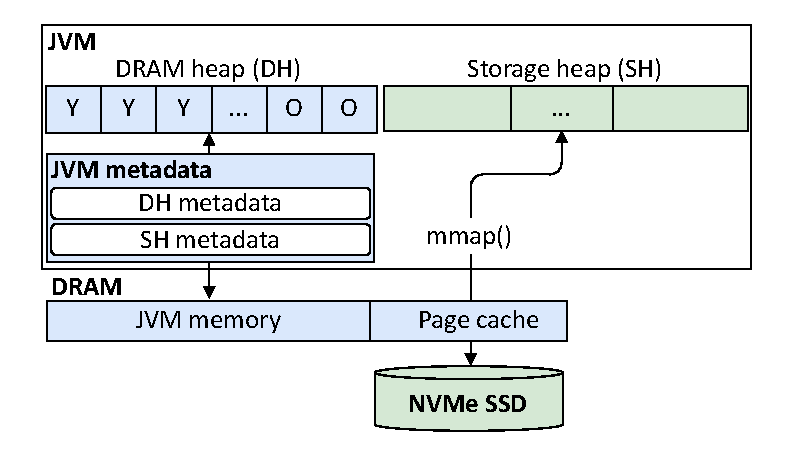
\includegraphics[width=0.6\linewidth]{chipper/figures/design/overview.pdf}
	\caption{\chipperName{} design overview (acronyms: \textbf{Y=}\textbf{Y}oung generation region, \textbf{O=}\textbf{O}ld generation region).}
	\label{fig:over}
\end{figure}

Next, we describe how we design \chipperName{} to work with the three main aspects of low-pause collectors: (1) bounding GC work (\S\ref{sec:distribute}), (2) parallel object evacuation (\S\ref{sec:evacuate}), and (3) separate handling of large objects (\S\ref{sec:nonmovable}).
Finally, we describe how \chipperName{} reclaims space in SH (\S\ref{sec:sh-reclaim}).

\subsection{Bounding GC Work}
\label{sec:distribute}

\chipperName{}'s main function is to migrate objects from DH to SH, allowing the application heap and its result caches to grow beyond the available DRAM.
We refer to objects evacuated during incremental GCs as \emph{regular objects}.
For regular objects, SH migration changes both the amount of DH space reclaimed from a region and the evacuation work required to reclaim that DH space.
Ignoring the additional DH space reclaimed by SH migration can delay migration, while ignoring SH evacuation work can cause the collector to exceed the intended GC work budget.
\chipperName{} therefore extends the collector's region-efficiency model to account for both the DH space reclaimed by SH migration and the corresponding evacuation cost as follows:
%
\begin{equation}
	E(r) = \frac{R_{DH}(r)} {W_{\mathit{evac}}(r)},
\end{equation}
%
where $R_{DH}(r)$ is the DH space reclaimed by evacuating region $r$, and $W_{\mathit{evac}}(r)$ is the corresponding evacuation work.
A higher region efficiency identifies a region that reclaims more DH space for the same evacuation work, or requires less evacuation work to reclaim the same amount of DH space.

\paragraph{\textbf{Estimating reclaimed DH space.}}
Estimating the DH space that a region reclaims requires knowing which of its live objects migrate to SH.
For this object selection, \chipperName{} adopts mechanisms from prior work~\cite{wang:bridgegc,khanh:yak,teraheap,leaksurvivor, kolokasis:teracache,bond:melt,khanh:polar}.
An application labels a cache root object at runtime, and \chipperName{} propagates the label to the objects in its transitive closure during concurrent marking.
We call a labeled object an \emph{SH candidate}.
Live SH candidates contribute to reclaimed DH space even though the SH candidates are not garbage.
After migration to SH, the DH space occupied by an SH candidate becomes available for reuse.
\chipperName{} therefore computes
%
\begin{equation}
	R_{DH}(r) = G(r) + L_{SH}(r),
\end{equation}
%
where, in region $r$, $G(r)$ is the amount of garbage and $L_{SH}(r)$ is the volume of live bytes selected for SH migration.
The remaining live bytes, which are evacuated within DH, are denoted by $L_{DH}(r)$.

Region selection occurs after concurrent marking, so $L_{SH}(r)$ must be available when concurrent marking completes.
\chipperName{} therefore computes $L_{SH}(r)$ during concurrent marking, while the collector scans the object graph to identify live objects.
Similar to prior work~\cite{wu:espresso,teraheap}, \chipperName{} maintains a 64-bit SH-candidate field in each object's header to record whether the object is selected for SH migration.
When concurrent marking identifies a live SH candidate, \chipperName{} adds the object's size to a counter associated with the object's DH region.
At the end of concurrent marking, the counter gives $L_{SH}(r)$, while the remaining live bytes constitute $L_{DH}(r)$.

\chipperName{} does not require all objects in a labeled root's transitive closure to be identified during the same concurrent marking cycle.
An object not identified as an SH candidate during the current concurrent marking cycle remains in DH and may be identified during a later concurrent marking cycle.
Delayed SH-candidate identification affects only SH migration progress; object liveness remains governed by the collector's existing scanning and barrier mechanisms.

\paragraph{\textbf{Estimating evacuation work.}}
Evacuating an object to SH may cost more than evacuating the object within DH because the copy goes through the OS page cache, and the SH evacuation cost depends on whether the target pages are resident.
\chipperName{} therefore computes
%
\begin{equation}
	W_{\mathit{evac}}(r) = C_{DH} \cdot L_{DH}(r) + C_{SH} \cdot L_{SH}(r),
\end{equation}
%
where $C_{DH}$ is the estimated per-byte cost of evacuation within DH, and $C_{SH}$ is the estimated per-byte cost of evacuation from DH to SH.

The per-byte cost of evacuation to SH depends on the state of the OS page cache, so \chipperName{} cannot derive $C_{SH}$ statically.
\chipperName{} therefore estimates $C_{DH}$ and $C_{SH}$ from evacuation measurements.
For each destination, \chipperName{} divides the aggregate evacuation time across GC threads by the total number of bytes evacuated to that destination.
The SH evacuation measurement includes the mmio copy and any synchronous delays incurred through the OS page cache.
For example, accessing a non-resident SH page may trigger a page fault, while OS page-cache pressure may delay a GC thread while the kernel makes page-cache space available.

After each GC that performs SH evacuation, \chipperName{} computes a new per-byte SH evacuation-cost sample and smooths $C_{SH}$ over recent samples to avoid reacting to individual I/O variations.
Before observing the first SH evacuation, \chipperName{} initializes $C_{SH}$ to $C_{DH}$.

\chipperName{} does not prescribe how a collector selects regions for evacuation.
Instead, \chipperName{} provides SH-aware estimates of the DH space reclaimed from each region and the evacuation work required to reclaim that DH space.
A low-pause collector uses the SH-aware estimates to rank regions and to predict the evacuation work of the regions admitted into an incremental GC.

\subsection{Parallel Object Evacuation}
\label{sec:evacuate}

\chipperName{} must preserve evacuation parallelism when migrating objects to SH.
The label of an SH candidate determines the SH region that receives the object, so that \chipperName{} collocates the objects of a cache in SH.
A GC thread may therefore evacuate objects of different labels into different SH regions during one GC, which per-thread allocation state cannot serve: maintaining separate allocation state for every GC thread and for every active SH region would increase DRAM metadata.
\chipperName{} therefore associates an allocation lock with each label-to-region mapping.
GC threads targeting different labels can allocate from different current SH regions in parallel, while GC threads targeting the same label serialize allocation.

\begin{figure}[t]
	\centering
	\subfloat[]{%
		\begin{minipage}[b][5.5cm][c]{0.375\linewidth}
			\centering
			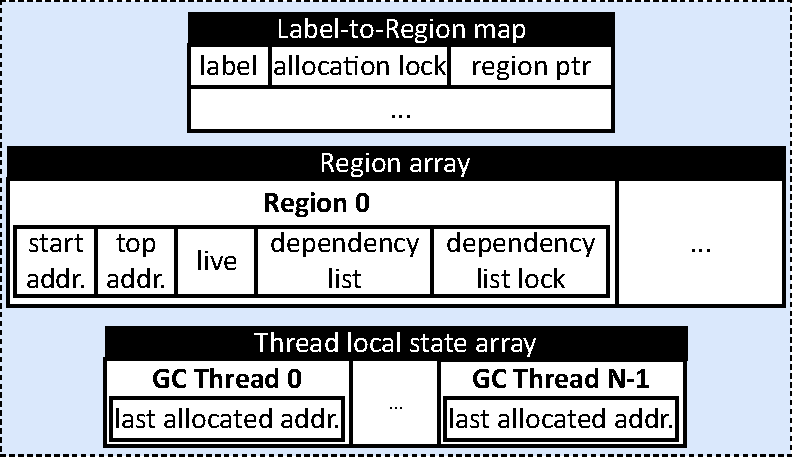
\includegraphics[width=\linewidth]{chipper/figures/design/allocator_meta.pdf}
		\end{minipage}
	}
	\hfill
	\subfloat[]{%
		\begin{minipage}[b][5.5cm][c]{0.6\linewidth}
			\centering
			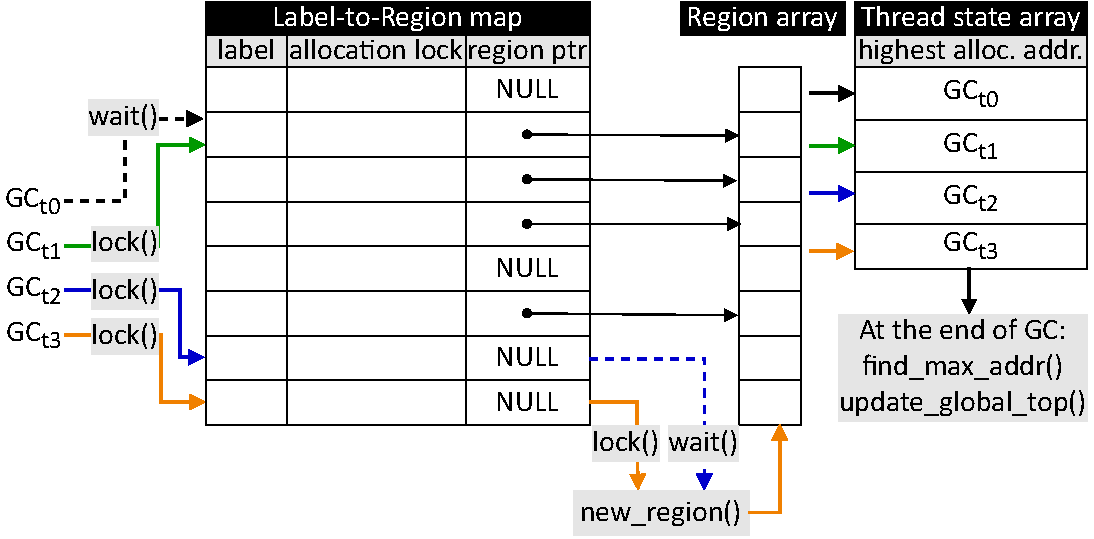
\includegraphics[width=\linewidth]{chipper/figures/design/parallel-allocator.pdf}
		\end{minipage}
	}
	\caption{(a) SH allocator metadata in DRAM and (b) parallel evacuation across multiple SH regions.}
	\label{fig:alloc-meta}
\end{figure}

Figure~\ref{fig:alloc-meta}(a) shows the SH allocator metadata that \chipperName{} maintains in DRAM.
Each entry in the Label-to-Region map contains an allocation lock and a pointer to the current SH region for the corresponding label.
The metadata of each SH region records the allocation position.
Allocating space for an object in SH proceeds in two steps.
First, a GC thread acquires the allocation lock for the label, reserves space in the current SH region, advances the allocation position, and releases the lock.
Second, the GC thread updates its thread-local state to record the highest SH address it has allocated.
At the end of the GC, \chipperName{} determines the highest allocated address across all GC threads and updates the global SH top address if it is lower than this address.
This avoids synchronization on the update of the SH global top address during parallel evacuation.

Figure~\ref{fig:alloc-meta}(b) illustrates how this design enables parallel allocation across multiple SH regions.
GC threads allocating objects with different labels acquire independent allocation locks and can reserve space concurrently.
In contrast, threads allocating objects with the same label must wait for the corresponding allocation lock.
Assigning a new SH region to a label requires global synchronization because the operation modifies the free-region pool shared by all labels.
When a label has no current SH region or the current region lacks sufficient free space, the GC thread acquires the global lock, allocates a new SH region from the free-region pool, and updates the region pointer in the corresponding Label-to-Region map entry.
As illustrated in Figure~\ref{fig:alloc-meta}(b), GC threads $t_2$ and $t_3$ allocate objects with different labels but contend for the \emph{global region allocation lock} because both need to assign a new SH region.
Thus, synchronization is limited to space reservation among threads sharing the same label and global region assignment, allowing allocations to existing regions with different labels to proceed independently.

Evacuation to SH also constrains the collector's forwarding mechanism.
The complete object must be available at the SH destination before the collector publishes that address as the forwarding destination.
Prior storage-backed heaps may stage objects in intermediate DRAM buffers and write the objects asynchronously to storage~\cite{bond:melt,teraheap}.
An intermediate DRAM buffer cannot serve as the final SH destination for collectors that evacuate concurrently with mutators, such as ZGC and Shenandoah, because mutators may access an object immediately after the forwarding destination is published.
\chipperName{} instead uses mmio to copy the object directly to the final SH address through the OS page cache.
After the mmio copy completes, the collector can publish the SH address as the forwarding destination without waiting for dirty pages to be written to the NVMe device; the kernel performs dirty-page write-back later.
For STW collectors, intermediate DRAM buffers are safe while mutators remain stopped, but the GC pause cannot end until all objects are drained from the intermediate buffers and copied to their final SH destinations.

\paragraph{\textbf{Handling concurrent evacuation of the same object.}}
Multiple GC threads may encounter the same SH candidate through different references and attempt to evacuate the object concurrently.
Each GC thread may reserve a different SH destination.
The collector's forwarding mechanism ensures that only one reserved SH destination becomes the object's forwarding destination.
A GC thread whose reserved destination is not selected fills the unused allocation range with a filler object, allowing subsequent SH card scanning to traverse the SH region linearly.
Concurrent evacuation of the same object may therefore consume additional SH space, but avoids additional synchronization on the object-evacuation path.
We quantify this space overhead in \S\ref{chipper:sec:eval}.

\subsection{Handling Large Objects}
\label{sec:nonmovable}

Incremental GCs do not evacuate large objects, so a large SH candidate cannot leave DH through an incremental GC and occupies DRAM while it is live.
Its migration therefore requires a GC that evacuates objects without a GC work budget.
\chipperName{} identifies large SH candidates during concurrent marking, as it does for regular objects, and preserves the SH-candidate state across GCs.
When the collector invokes its mechanism for relieving memory pressure, \chipperName{} migrates the retained large SH candidates.

Migrating a large SH candidate is safe only after the complete object is available at its SH destination and references can resolve to that destination.
\chipperName{} therefore assigns each live large SH candidate an SH destination, integrates the SH destination with the collector's forwarding and reference-update mechanisms, and reclaims the original DH space only after migration completes.
If the collector does not invoke the mechanism for relieving memory pressure, the large SH candidate remains in DH and migration is deferred.

\paragraph{\textbf{Preserving SH-to-DH (backward) references to deferred large objects.}}
Backward references can arise from partial migration of a labeled object graph or from mutator updates.
Regular objects may migrate to SH during incremental GCs while referenced large SH candidates remain in DH awaiting migration.
This partial migration creates backward references from migrated SH objects to large SH candidates that remain in DH.
Mutators may also create new backward references by storing a DH reference into an SH object.
The collector must observe both sources of backward references to preserve the liveness of referenced DH objects and to update the backward references when referenced DH objects move.

Similar to previous work~\cite{teraheap,kolokasis:teraheap_toplas}, \chipperName{} tracks backward references using an SH card table maintained in DRAM, with one byte for each fixed-size segment of SH.
To detect backward references created by mutators, \chipperName{} extends the post-write barrier emitted by the interpreter and the C1 and C2 JIT compilers.
The post-write barrier marks the corresponding SH card \emph{dirty} whenever a mutator updates a reference field in an SH object.
During a GC, GC threads scan dirty SH cards in parallel and process backward references as GC roots.
If a referenced DH object is evacuated, \chipperName{} updates the backward reference to the object's forwarding destination.

Scanning SH cards may access storage-resident objects and incur storage I/O.
To avoid rescanning SH cards whose backward references are irrelevant to a GC, \chipperName{} classifies each scanned SH card according to the referenced DH objects.
For generational collectors, an SH card becomes \emph{clean} if the card contains no backward references, \emph{old} if all backward references point to old generation objects, and \emph{young} if at least one backward reference points to a young generation object.
A young GC can therefore skip clean and old SH cards and scan only SH cards that may contain references relevant to the collection.

Skipping an old SH card is safe only when an incremental GC cannot reclaim an old object referenced by that card.
Large objects require special treatment because a collector may reclaim a dead large object during an incremental GC without evacuating the object.
For example, G1 eagerly reclaims dead large objects during young GCs.
If a backward reference is the only reference keeping a large SH candidate live, skipping the corresponding SH card would hide the backward reference from the collector and could cause premature reclamation.
\chipperName{} therefore classifies an SH card that references a large SH candidate awaiting migration as \emph{young}, regardless of the large object's generation.
The SH card remains \emph{young} until the referenced large SH candidate is migrated to SH or becomes dead.

\subsection{Reclaiming SH Space}
\label{sec:sh-reclaim}

Like prior storage-backed heaps~\cite{leaksurvivor,teraheap}, \chipperName{} reclaims an SH region only when all objects in the region are dead, trading SH capacity for storage I/O.
Reclaiming a partially live SH region would require evacuating the live objects in the region, generating additional storage I/O that can increase application latency.

\paragraph{\textbf{Tracking SH inter-region references.}}
The collector does not scan SH objects during concurrent marking, so SH-region liveness cannot be determined by following references between SH regions directly.
We refer to an SH-to-SH reference whose source and target objects reside in different SH regions as an \emph{inter-region reference}.
Similar to TeraHeap~\cite{teraheap}, \chipperName{} maintains a dependency list for each SH region.
The dependency list records the target SH regions of inter-region references originating from the corresponding source SH region, as shown in Figure~\ref{fig:alloc-meta}(a).
During concurrent marking, \chipperName{} uses these SH-region dependencies to propagate liveness across SH regions without scanning SH objects.

\chipperName{} records SH-region dependencies when inter-region references are created during object evacuation or by mutator updates.
When an object is evacuated to SH, \chipperName{} examines the object's references to SH objects.
For each inter-region reference, \chipperName{} adds the target SH region to the dependency list of the object's destination SH region if the dependency is not already present.
A mutator may subsequently create a new inter-region reference by updating a reference field in an SH object.
When GC threads scan the corresponding dirty SH card, \chipperName{} adds the target SH region to the dependency list of the source SH region if the dependency is not already present.

Multiple GC threads may update dependency lists concurrently.
Each SH region therefore maintains a dependency lock separate from the allocation lock described in \S\ref{sec:evacuate}.
GC threads updating different dependency lists proceed in parallel, while GC threads updating the same dependency list synchronize using the corresponding dependency lock.

\paragraph{\textbf{Reclaiming SH regions.}}
To reclaim SH regions without scanning SH objects, \chipperName{} tracks SH-region liveness using DRAM metadata.
Each SH region maintains a liveness bit in its DRAM metadata, as shown in Figure~\ref{fig:alloc-meta}(a).
At the beginning of concurrent marking, \chipperName{} clears the liveness bit of every allocated SH region.
When concurrent marking encounters a DH-to-SH reference, \chipperName{} sets the liveness bit of the referenced SH region and propagates liveness transitively through the region's dependency list.
Consequently, an SH region becomes live only when the region is reachable from DH, directly or through another live SH region.
Mutually referencing dead SH regions therefore remain dead.

Prior storage-backed heaps determine SH-region liveness while mutators are stopped, whereas \chipperName{} determines SH-region liveness concurrently with mutators.
Concurrent marking must therefore account for the references that mutators overwrite while marking is in progress.
Low pause collectors use snapshot-at-the-beginning (SATB) marking: a barrier records every reference that a mutator overwrites during concurrent marking, and the collector processes the recorded references as part of marking, so that an object reachable when marking began remains live for the marking cycle.
\chipperName{} also processes the DH-to-SH references that the SATB barrier records, so that an SH region reachable when marking began remains live even if a mutator overwrites the last DH reference to it.
% Before finalizing SH-region liveness, \chipperName{} processes SH cards dirtied
% during concurrent marking to account for SH-to-SH references created by mutator
% updates.

At the end of concurrent marking, \chipperName{} examines the liveness bit of every allocated SH region.
An SH region whose liveness bit remains clear contains no live objects, so \chipperName{} resets the region's metadata and makes the entire SH region available for reuse without scanning the region's objects.
SH-region liveness is conservative: a dead SH object remains allocated until every object in the same SH region is dead.
This conservatism affects SH capacity but not correctness.
